\documentclass[11pt,a4paper]{article}
\usepackage[russian]{babel}
\usepackage[utf8]{inputenc}
\usepackage{amsmath}
\usepackage{mathtools} 
\usepackage[russian]{babel}
\usepackage{hyperref}
\usepackage{amssymb}
\usepackage{multicol}
\usepackage{bm}
\usepackage[hcentering, bindingoffset = 10mm, right = 15 mm, left = 15 mm, top=20mm, bottom = 20 mm]{geometry}
\newcounter{prim}
\newenvironment{prim}{%
	\addtocounter{prim}{1}
	\noindent{\\
		\textbf{\noindentПример \arabic{prim}\\}}%
}{}

\DeclareMathOperator{\tr}{\mathop{tr}}
\DeclareMathOperator{\Ker}{\mathop{Ker}}
\DeclareMathOperator{\im}{\mathop{Im}}
\DeclareMathOperator{\const}{\mathop{const}}
\DeclareMathOperator{\rg}{\mathop{rg}}
\newtheorem{definition}{Определение}[section]
\newtheorem{theorem}{Теорема}[section]
\renewcommand{\labelenumi}{\asbuk{enumi})}

\begin{document}
	\part*{Лабораторная работа 3.2.6}
	\part*{Исследование гальванометра}
	\textbf{Работу выполнили:} \\
	{\itshape Морозов Матвей \\ Бабушкина Татьяна \\ 678 группа} \\\\
\textbf{Цель работы:} изучение работы высокочувствительного зеркального гальванометра магнитоэлектрической системы в режимах измерения постоянного тока и электрического тока.
\\\\
\textbf {В работе используются:} зеркальный гальванометр с осветителем и шкалой, источник постоянного напряжения, делитель напряжения, магазин сопротивлений, эталонный конденсатор, вольтметр, переключатель, ключи, линейка.
\\
\\
\part*{Теоретическая часть}
Баллистическим гальванометром называют электроизмерительный прибор магнитоэлектрической системы, отличающийся высокой чувствительностью к току и сравнительно большим периодом колебаний подвижной системы (рамки). \\\
Баллистический гальванометр позволяет измерять как постоянный ток - стационарный режим, так и заряд, протекший через рамку за некоторое время - баллистический режим.\\
\textbf{Уравнение движения подвижной системы}\\
На рамку в магнитном поле действует моменты сил: момент закрученной нити, момент магнитных сил и тормозящий момент. 
\\
\\
Механический момент: $M_1 = -D\varphi$, где $D$ - модуль кручения нити, $\varphi$ - угол поворота рамки от положения равновесия.\\
\\
Момент магнитных сил: $M_2=2rlBNI=BSNI$, где $r$ - расстояние от боковой стороны до оси вращения, $S$ - площадь одного витка, $N$ - количество витков, $I$ - ток.\\
\\
Тормозящий момент: $M_3 = BSNI_i=- \cfrac{(BSN)^2}{R_\sigma}\varphi^\cdot$, где $I_i$ - индукционный ток.\\
\\
Уравнение движения рамки имеет вид: $J\varphi^{..} = \Sigma M$, подставим сумму моментов всех сил, действующих на рамку, и получим: $J\varphi^{..} + \cfrac{(BSN)^2}{R_\sigma}\varphi^\cdot + D\varphi = BSNI$\\
\\
Уравнение движения рамки примет вид: $\varphi^{..} + 2\gamma \varphi^{.} + w_0^2\varphi = KI$, где $\gamma$ - коэффициент затухания, $w_0$ - собственная частота колебаний рамки.\\
\\
\textbf{Режим измерения постоянного тока}\\
\\
$\varphi = \cfrac{K}{w_0^2}I = \cfrac{BSN}{D}I = \cfrac{I}{C_I}$, где $C_I$ - динамическая постоянная.\\
\\
\textbf{Свободные колебания рамки}\\
\\
В начальный момент времени $\varphi^{..} + 2\gamma \varphi^{.} + w_0^2\varphi = 0$\\
\\
Общее решение:$\varphi = A_1e^{\lambda_1t} + A_2e^{\lambda_2t}$, далее возможны три варианта: \\
1) Колебательный режим: $\gamma < w_0$, $\varphi = \frac{\varphi^{.}}{w_0} sin w_0t$\\
2) Критический режим : $\gamma < w_0$, $\varphi = \varphi^{.}te^{-\gamma t}$\\
3)Затухание :$\gamma > w_0$, $\varphi = \cfrac{\varphi ^.}{\varkappa}e^{ - \gamma t} sh \varkappa t$\\

\textbf{Определение динамической постоянной}\\

При малых $R_1$ сила тока, протекающего через гальванометр может быть вычислена по очевидной формуле: $I = U_0 \cfrac{R_1}{R_2} \cfrac{1}{R_0 + R}$, где $U_0$ - показания вольтметра, $\cfrac{R_1}{R_2}$ - положение делителя, $R$ -- сопротивление магазина, $R_0$ -- внутреннее сопротивление гальванометра.\\
\\
Координата $x$ светового пятна на шкале связана с углом отклонения рамки формулой $x = a tg(2 \varphi)$, где $a$ расстояние от шкалы до зеркальца. $C_I =\cfrac{I}{\varphi} = \cfrac{2aI}{x}.$\\
\\

\textbf{Определение критического сопротивления гальванометра}\\
\\
Скорость затухания колебаний принято характеризовать декрементом затухания $\Delta$, равным отношению углов двух последовательных отклонений в одну сторону. $\Delta = \cfrac{\varphi_n}{\varphi_{n+1}} = e^{\gamma t}$, где $T = \cfrac{2 \pi}{w}$.\\
Мы будем рассматривать логарифмический декремент затухания $\theta = ln \Delta = \gamma T = ln \cfrac{x_n}{x_{n+1}}$\\
Измеряя зависимость логарифмического декремента затухания от сопротивления внешней цепи, можно найти $R_k$ - критическое сопротивление,  при котором $\theta = \infty$ : $R_k = \cfrac{1}{2 \pi} \sqrt{\cfrac{X}{Y}} - R_0$, где $X = (R + R_0)^2$, $Y = \cfrac{1}{\theta^2}$
\\
\\
\textbf{Определение баллистической постоянной и критического сопротивления гальванометра, работающего в баллистическом режиме}\\
\\
При нормальном положении кнопки $K_0$ конденсатор $C$ заряжается до напряжения $U_C = \cfrac{R_1}{R_2}U_0$, заряд конденсатора равен $q = C U_C = \cfrac{R_1}{R_2}U_0 C$.\\
\\
Баллистическая постоянная определяется при критическом сопротивлении ($R_k= R$):\\ $C_Q = \cfrac{q}{\varphi_{max}} = 2a \cfrac{R_1}{R_2} \cfrac{U_0C}{l_{max}}$, где $l_{max}$ - величина первого отброса в критическомм режиме.

\part*{Обработка результатов}
\textbf{1)} Записали: \\\\
1) показание вольтметра $U_0 = 69 делений = 1,38 B$ \\
2) положение делителя $\frac{R1}{R_2} = \frac{1}{2000}$ \\
3) Величину $R_2 = 10 \text{кОм}$ \\
4) Внутреннее сопротивление $R_0 = 2000 \text{Ом}$, указанное на установке. \\\\
\textbf{2)} Рассчитаем токи $I$ по формуле $I = U_{0} \cfrac{R_1}{R_2} \cfrac{1}{R+R_0}$
\\

\begin{table}[h!]
	\begin{center}
		\textbf{Таблица 1}. Зависимость $I$ от $x$.\\
	\begin{tabular}{|c|c|c|c|c|c|c|c|c|}
		
			\hline
			№ & $x, \text{ см}$        & $R, \text{ Ом}$  & $I, \text{ нА}$ && № & $x, \text{ см}$        & $R, \text{ Ом}$  & $I, \text{ нА}$ \\ \hline
			\textbf{1} & $24,5$ & $10009,9$ & $57,452$ & &\textbf{15} & $11,5$ & $29900,0$ & $21,630$\\ \hline
			\textbf{2} & $23,0$ & $11009,9$ & $53,037$ & &\textbf{16} & $10,8$ & $31900,0$ & $20,354$ \\ \hline
			\textbf{3} & $21,9$ & $12109,9$ & $48,902$ & &\textbf{17} & $9,9$ & $33900,0$ & $19,220$ \\ \hline
			\textbf{4} & $21,0$ & $13109,9$ & $45,665$ & &\textbf{18} & $8,9$ & $36900,0$ & $17,738$ \\ \hline
			\textbf{5} & $20,0$ & $14109,9$ & $42,831$ & &\textbf{19} & $8,1$ & $38900,0$ & $16,687$ \\ \hline
			\textbf{6} & $19,0$ & $15309,9$ & $39,861$ & &\textbf{20} & $7,4$ & $41900,0$ & $15,717$ \\ \hline
			\textbf{7} & $18,0$ & $16909,9$ & $36,489$ & &\textbf{21} & $6,5$ & $45900,0$ & $14,405$ \\ \hline
			\textbf{8} & $17,0$ & $18609,9$ & $33,479$ & &\textbf{22} & $5,9$ & $49900,0$ & $13,295$ \\ \hline
			\textbf{9} & $15,4$ & $21900,0$ & $28,870$ & &\textbf{23} & $5,2$ & $54700,0$ & $12,169$\\ \hline
			\textbf{10} & $14,7$ & $22999,0$ & $27,601$ & &\textbf{24} & $4,5$ & $61700,0$ & $10,832$ \\ \hline
			\textbf{11} & $14,2$ & $23900,0$ & $26,641$ & &\textbf{25} & $3,9$ & $68700,0$ & $9,759$\\ \hline
			\textbf{12} & $13,4$ & $25900,0$ & $24,731$ & &\textbf{26} & $3,4$ & $79700,0$ & $8,446$ \\ \hline
			\textbf{13} & $12,5$ & $27900,0$ & $23,077$ & &\textbf{27} & $2,9$ & $89700,0$ & $7,525$  \\ \hline
			\textbf{14} & $12,0$ & $28900,0$ & $22,330$ & &\textbf{28} & $2,5$ & $99909,9$ & $6,771$ \\ \hline		
	\end{tabular}
	\end{center}
\end{table}
\space
\textbf{3)} Построим графих зависимости $I(x)$

\begin{figure}[h!]
		\centering
		\textbf{График 1}\\
	Зависимость $I(x)$
	\\

	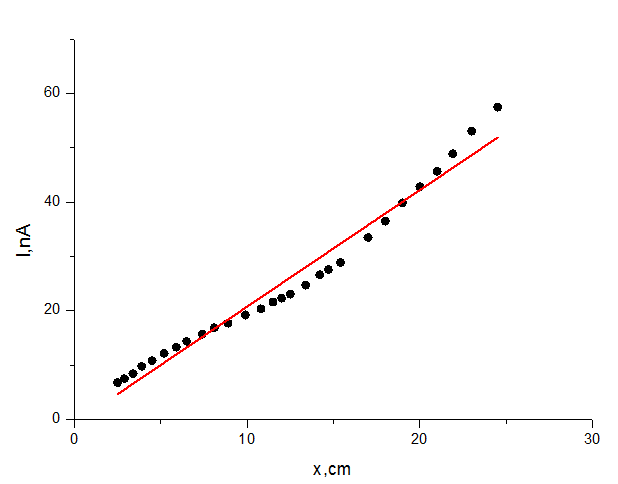
\includegraphics[width=0.7\linewidth]{20}

\end{figure}
При помощи метода наименьших квадратов (МНК) рассчитаем тангенс наклона прямой на графике $1$. 
\\
Тангенс наклона можно посчитать по формуле: $k = \frac {<xI> - <x><I>}{<x^2> - <x>^2}$.
\\
Погрешность тангенса наклона посчитаем по формуле: $\delta k = \frac{1}{\sqrt{n}} \sqrt{\frac{<I^2> - <I>^2}{<x^2> - <x>^2} - k^2}$
\\
Получили: $k = (2,14 \pm 0,07) \cdot 10^{-7} \frac{\text{A}}{\text{м}}$ \\\\
Посчитаем динамическую постоянную $C_I$ по формуле $C_I = 2ak$, где $a = 1,1  \text{м}$ - расстояние от шкалы до зеркальца гальвонометра.
\\\\
Получили: $\boxed {C_I = (4,71 \pm 0,15) \cdot 10^{-10} \frac{\text{A}}{\text{мм} / \text{м}}}$
\\\\
\textbf{4)} Рассчитаем логарифмический декремент затухания $\Theta_0$ разомкнутого гальвонометра по формуле $\Theta = \ln \frac{x_n}{x_{n+1}}$.
\\

\begin{table}[h!]
	\begin{center}
		\textbf{Таблица 2}.Расчёт $\Theta_0$\\
		\begin{tabular}{|c|c|c|c|c|c|c|c|c|c|c|}
			
			\hline
			$x_1,\text{см}$ & $24,0$  & $21,8$ & $19,9$ & $18,1$ & $16,6$ & $14,9$ & $13,5$ & $12,1$  & $11,0$ & $9,8$ \\ \hline
			$x_2,\text{см}$ & $21,8$ & $19,9$ & $18,1$ & $16,6$ & $14,9$ & $13,5$ & $12,1$  & $11,0$ & $9,8$ & $8,9$ \\ \hline
			$\theta_0$ & $0,096$ & $0,091$ & $0,095$ & $0,087$ & $0,108$ & $0,099$ & $0,109$  & $0,095$ & $0,116$ & $0,096$ \\ \hline
	\end{tabular}
\end{center}
\end{table}
$\boxed{\Theta_0 = 0,099}$ \\\\
\textbf{5)}
\begin{table}[h!]
	\begin{center}
		\textbf{Таблица 3} \\
		Зависимость $\frac{1}{\Theta^2}$ от $(R+R_0)^2$.\\
		\begin{tabular}{|c|c|c|c|c|c|}
			\hline
		 $R, \text{Ом}$ & $x_1, \text{см}$ &$x_2, \text{см}$ & $\Theta$ & $\frac{1}{\Theta^2}$ & $(R+R_0)^2, \text{кОм}$ \\ \hline
			$43000$ &	$15,5$ & $1,4$ & $2,404$ & $0,173$ & $2025$ \\ \hline
			$48000$	& $14,1$ & $1,6$ & $2,176$ & $0,211$ & $2500$ \\ \hline
			$53000$	& $13,1$ & $1,9$ & $1,931$ & $0,268$ & $3025$ \\ \hline
			$58000$	& $11,9$ & $2,0$ & $1,783$ & $0,314$ & $3600$ \\ \hline
			$63000$	& $10,9$ & $2,1$ & $1,647$ & $0,369$ & $4225$ \\ \hline
			$68000$	& $10,0$ & $2,1$ & $1,561$ & $0,411$ & $4900$ \\ \hline
			$73000$	& $9,0$ &  $2,2$ &$1,409$	& $0,504$ & $5625$ \\ \hline
			$78000$	& $8,2$ & $2,1$ & $1,362$ & $0,539$ & $6400$ \\ \hline
			$83000$	& $7,5$ & $2,1$ & $1,273$ & $0,617$ & $7225$ \\ \hline
			$88000$	& $6,8$	& $2,1$ & $1,175$ & $0,724$ & $8100$ \\ \hline
			$93000$	& $6,4$ & $2,1$ & $1,114$ & $0,805$ & $9025$ \\ \hline
		\end{tabular}
	\end{center}
\end{table}
Построим график $\frac{1}{\Theta^2} = f[(R+R_0)^2]$ и по наклону прямой (в области малых $R$) рассчитаем критическое сопротивление по формуле:
$R_{\text{кр}} = \frac{1}{2\pi} \sqrt{\frac{\Delta X}{\Delta Y}} - R_0$ \\
\begin{figure}[h!]
	\centering
\textbf{График 2}\\
Зависимость  $\frac{1}{\Theta^2}$ от $(R+R_0)^2$
\\
	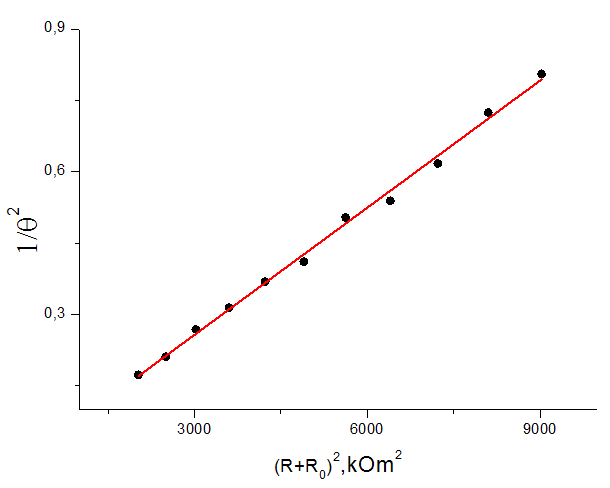
\includegraphics[width=0.5\linewidth]{22}
\end{figure}
\newpage
При помощи метода наименьших квадратов (МНК) рассчитаем тангенс наклона прямой на графике $2$. \\
\\
Тангенс наклона можно посчитать по формуле: $k = \cfrac {< \cfrac{1}{\Theta^2}(R+R_0)^2 > - <\cfrac{1}{\Theta^2}><(R+R_0)^2>}{<(R+R_0)^4> - <(R+R_0)^2>^2}$.
\\\\
Погрешность тангенса наклона посчитаем по формуле: $\delta k = \cfrac{1}{\sqrt{n}} \sqrt{\cfrac{<(\frac{1}{\Theta^2})^2> - <\frac{1}{\Theta^2}>^2}{<(R+R_0)^4> - <(R+R_0)^2>^2} - k^2}$ \\\\
Получили: $k = (8,91 \pm 0,18) \cdot 10^{-5}, \text{кОм}^2$ \\\\
$R_{\text{кр}} = \cfrac{1}{2\pi} \sqrt{\cfrac{1}{k}} - R_0$\\\\
$\boxed{R_{\text{кр}} = (14,86 \pm 1,04) \ \ \text{кОм}}$ \\\\
\textbf{6)} Измерили максимальное отклонение при разомкнутой цепи $L_{max_1} = 18 \ \ \text{см}$.

\begin{table}[h!]
	\begin{center}
		\textbf{Таблица 4} \\
		Зависимость первого отброса $l_{max}$ от $(R+R_0)^2$.\\
		\begin{tabular}{|c|c|c|}
			\hline
$l_{max}, \text{см}$ & $R, \text{Ом}$	& $(R+R_0)^{-1}, \frac{10^{-6}}{\text{Ом}}$ \\ \hline
$12,2$ & $50000$ &	$19,23$ \\ \hline
$11,8$ & $45000$ &	$21,28$ \\ \hline
$10,6$ & $40000$ &	$23,81$ \\ \hline
$10,7$ & $35000$ &	$27,03$ \\ \hline
$9,6$  & $30000$ &	$31,25$ \\ \hline
$9,4$  & $25000$ &	$37,04$ \\ \hline
$8,5$  & $20000$ &	$45,45$ \\ \hline
$7,6$  & $15000$ &	$58,82$ \\ \hline
$5,6$  & $10000$ &	$83,33$ \\ \hline
$4,5$  & $5000$  &	$142,86$ \\ \hline
		\end{tabular}
\end{center}
\end{table}
Построим график зависимости $l_{max} = f[(R+R_0)^{-1}]$ и определим по графику критическое сопротивление гальванометра с учётом формулы:\\\\
$\varphi_0 = \varphi_1 \cdot \exp (\Theta_0/4)$, где \\
$\Theta_0$ -- логарифмический декремент затухания; \\
$\varphi_1$ -- максимальное отклонение рамки при размокнутой цепи; \\
$\varphi_0$ -- максимальное отклонение рамки при замкнутой цепи;
\newpage
\begin{figure}[h!]
		\centering
	\textbf{График 3}\\
	Зависимость $l_{max}$ от $(R+R_0)^{-1}$
	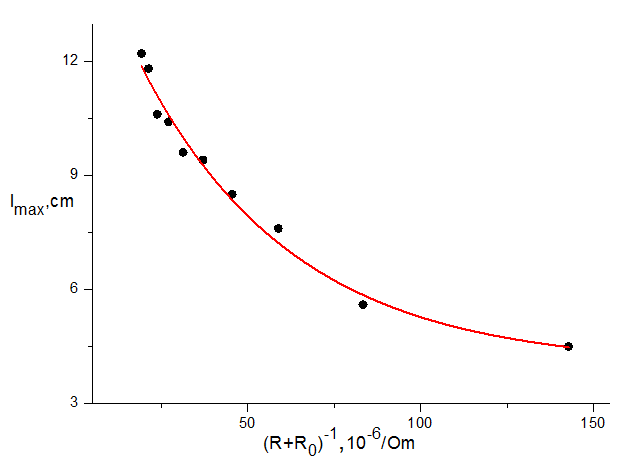
\includegraphics[width=0.7\linewidth]{23}
\end{figure}
Рассчитаем максимальное отклонение при свободных колебаниях $l_{max_0}$.
\\\\
$\varphi_1 = \arctan (\frac {l_{max_1}}{a})$ \\\\
$\varphi_0 = \arctan (\frac {l_{max_0}}{a})$ \\\\
$l_{max_0} = a \tan [\arctan(\frac{l_{max_1}}{a}) \exp (\Theta_0 / 4)] = 1,1 \cdot \tan (\arctan (18/110) \exp(0,18/4)) = 18,8 \ \ \text{см}$
\\\\
Максимальное отклонение в критическом режиме в $e$ раз меньше, чем при свободных колебаниях. \\
Получим: $l_{max_{\text{кр}}} = 6,9 \ \ \text{см}$. \\
Этому значению на графике соответствует $(R+R_0)^{-1} = 63,27 \ \ 10^{-6}/\text{Ом}$. Отсюда найдём критическое сопротивление: $R_{\text{кр}} = 13,8 \ \  \text{кОм}$.
\\\\
\textbf{7)} Cравним значения $R_{\text{кр}}$, определённые подбором и по графикам для стационарного и баллистического режима. \\\\
а) Определенное подбором: $R_{\text{кр}} = 14,31 \ \ \text{кОм}$ \\
б) Определенное по графику $2$ : $R_{\text{кр}} =  (14,86 \pm 1,04)\ \ \text{кОм}$ \\
в) Определенное по графику $3$ : $R_{\text{кр}} =  13,8 \ \ \text{кОм}$ \\\\
\textbf{8)} Рассчитайте баллистическую постоянную в критическом режиме $C_{Q_{\text{кр}}}$ [К/(мм/м)] 
по формуле $C_{Q_{\text{кр}}} = 2a \frac{R_1}{R_2} \frac {U_0 C}{l_{max \text{кр}}}$;\\\\
$C = 2 \cdot 10^{-6} \ \ \text{мкФ}$;\\\\
$\frac{R_1}{R_2} = \frac{1}{100}$;
\\\\
$C_{Q_{\text{кр}}} = 8,8 \cdot 10^{-10} \ \ \text{К/(мм/м)}$
\\\\
\textbf{9)} Сравним время релаксации $t = R_0 C$ и период свободных колебаний гальванометра $T_0$.
\\\\
$T_0 = 7,53 \ \ \text{с}$ \\
$t = 2000 \cdot 2 \cdot 10^{-6} = 4 \cdot 10^{-3} \ \ \text{с} $
\part*{Вывод}
\textbf{1)} Изучили работу зеркального гальванометра. \\\\
\textbf{2)} Определили динамическую постоянную $C_I = (4,71 \pm 0,15) \cdot 10^{-10} \frac{\text{A}}{\text{мм} / \text{м}}$ \\\\
\textbf{3)} Определили тремя способами критическое сопротивление гальванометра:\\\\
а) экспериментально : $R_{\text{кр}} = 14,31 \ \ \text{кОм}$ \\
б) статическим: $R_{\text{кр}} =  (14,86 \pm 1,04)\ \ \text{кОм}$ \\
в) баллистическим : $R_{\text{кр}} =  13,8 \ \ \text{кОм}$ \\\\
и они примерно совпадают.\\\\
\textbf{4)} Определили баллистическую постоянную $C_{Q_{\text{кр}}} = 8,8 \cdot 10^{-10} \ \ \text{К/(мм/м)}$
\\\\
\textbf{5)} Сравнили время релаксации $t$ и период свободных колебаний $T_0$ гальванометра.\\\\
$t = 4\cdot 10^{-3} \ \ \text{c}$; $T_0 = 7,53 \ \ \text{c}$; $t << T_0$.
\end{document}